Durant ces séances de TP, il nous a été demandé d'implémenter des fonctions capables de générer les maillages d'objets simples:

\textcolor{red}{ajouter sur les images des petites flèches pour montrer où est-ce qu'on a le tore, la sphère etc... plutôt que d'écrire du texte}
\textcolor{red}{rajouter deux icosphère avec différentes subdivisions pour montrer le travail}
\textcolor{red}{mettre côte à cote plusieurs images d'occlusion ambiante pour illustrer le travail --> différents nombre de samples pour le même nombre de vertex et différent nombre de vertex pour le même nombre de sample}
\textcolor{red}{comparer les perfs des intersections volumétriques avec les intersections de Mesh}


\begin {itemize}
	\item {Une sphere}
	\item {Un tore}
	\item {Une capsule}
	\item {Un cylindre}
\end {itemize}

Les maillages de ce projet utilisent des normales aux sommets simples qui ne produisent pas de maillage lisse.

\begin{figure}[h!]
	\adjustbox{center}{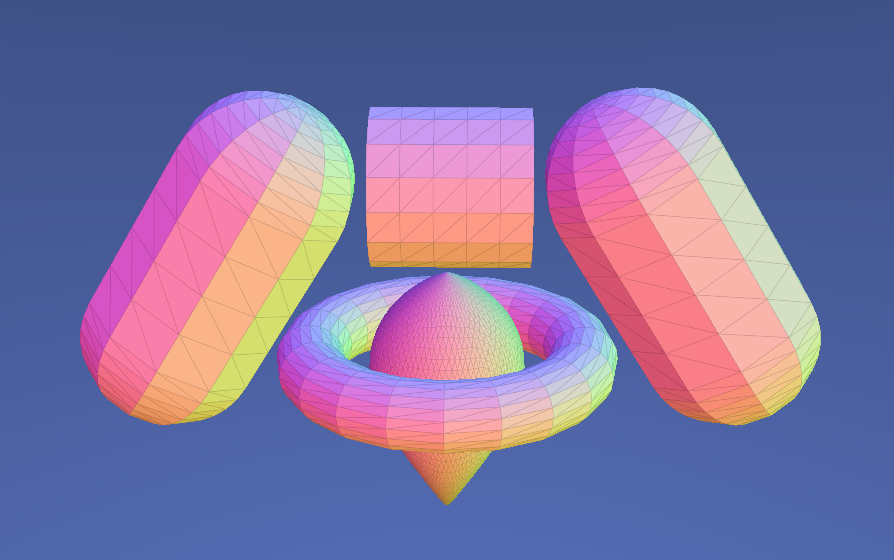
\includegraphics[width=0.75\textwidth]{Captures/transformations.png}}

	\caption{Union de maillages basiques. Les capsules ont été transformées par rotation et translation. L'icosphere au centre a été transformée par deux SphereWarp}
\end{figure}
\FloatBarrier
